\thesischapter{Simulating and Verifying the European Rail Traffic Management System Using Real Time Maude}\label{chapter:verifyertms}
In the following we describe how the Real Time Maude tool can be used to analyse the performance and safety of the ERTMS system by both simulation and verification using the Maude LTL model checker.  We begin by presenting the simulation of the pentagon example which demonstrates a situation where a slow train is held up by a faster train. Secondly we look at applying model checking to both the pentagon example and the junction example. The safety properties verified for the pentagon example relate to the safety condition "The movement authorities of the two trains do not overlap" whilst the properties for the junction example relate to the safety condition "The point does not move when it is in a trains movement authority".


It is stated by its developers that Real Time Maude is not first and foremost a verification tool. This is due to some inherent limitations in LTL-model checking that hinder the verification of infinite state systems. We have, as in the sensor network example \cite{PO07}, only model checked only a portion of the state space for the pentagon. This is however enough to have confidence in the correctness of the system with respect to a given safety condition. A larger portion of the state space could be model checked by removing non-determinism from the model and making it less loose. This has been done in the junction example where the radio block processor is forced to process movement authorities in one time step.


\section{Simulating The Behaviour of ERTMS}

We will now see how this executable specification can be used to simulate and analyse the perofrmanceof the modelled system. Simulation of the system up to a given time $n$ is achieved by rewriting the initial state of the system to each of the intermediate time steps $0 \ldots n$. A simple Haskell program has been written that can parse the output of each step, extract the relevant data and then plot a graph.

We use an initial state containing two trains one of which is slower (train1) than the other (train2), an interlocking and a radio block processor. The faster train will eventually catch up with the slow train and it waits for that train to clear all successive track segments before proceeding. The trains start at positions on opposing sides of the track with train1 starting at 0 and train2 starting at 150. The RBC and the interlocking are both initialised with the trains in these positions. In Maude this initial state is modelled as follows. Firstly, we define the initial states of the component objects individually:

\begin{lstlisting}[caption = The initial interlocking state in Maude]
 eq initialintstate2 = < inter1 : Inter | state : idle, 
                         reqid : 0, t0 : true, 
                         t1 : false, t2 : false, 
                         t3 : true, t4 : false > .
\end{lstlisting}

The  interlocking is initially idle, the request variable is set to zero, the track segments containing trains are set to true and the remaining track segments are set to false.

\begin{lstlisting}[caption = The initial RBC state in Maude]
 eq initialrbcstate2 = < rbc1 : RBC | state : rbcidle, 
                         lasttrain : train1,  
                         ma : (train1 |-> 49, train2 |-> 199), 
                         pos : (train1 |-> 0, train2 |-> 150), 
                         curreq : empty > .
\end{lstlisting}

Like the interlocking, the RBC is also initially idle. Since the lasttrain variable has not effect in this state and will be set in any successive control flow we simply set it to be train1. The movement authorites  and positions of the trains are set within the ma and pos mapping respectively and the current request is empty.  

\begin{lstlisting}[caption = The intital state of train2 in Maude]
 eq initialtrainstate1 = < train1 : Train | state : acc,  dist : 0, 
                           speed : 0, ac : 1, ma : 49, 
                           tseg : 0, maxspeed : 4 > .
\end{lstlisting}
We set the train1 to be accellerating initally with a distance and speed of zero its movement authority is fourty nine , it is in the zero track segment and has a maxspeed of four. 

\begin{lstlisting}[caption = The intial state of train2 in Maude]
eq initialtrainstate2  = < train2 : Train | state : acc, dist : 150, 
                           speed : 0, ac : 1, ma : 199,
                           tseg : 3, maxspeed : 7 > .
\end{lstlisting}
Like train1, train2 is also accellerating initially and has a speed of zero.  Unlike train1 it has a distance of one hundred and fifty, a movement authority of one hundred and ninty nine, it is in the fourth track segment number three and has a maxspeed of four. Both trains have an accelleration of one. 

Using these initial states for the individual objects we can form the initial state for our pentagon example using the following command:
\begin{lstlisting}
 eq initialstate2 = {initialtrainstate1 initialtrainstate2 
                         initialintstate2  initialrbcstate2} . 
\end{lstlisting}
The operation initial state 2 is of type System and contains a Configuration consisting of the initial states of train1, train2, the rbc and the interlocking. This initial state forms a model of ERTMS which we can simulate using Real Time Maude to rewrite it to a state after a set number of time steps. The model of ERTMS is executed using the following command:
\begin{center}
\texttt{(trew initialstate2 in time $\leq$ 50 .)}
\end{center}

In the resulting output at time 50 both of the trains have moved a considerable distance and have requested and received new movement authorities.
 
\begin{lstlisting}[caption = The result of rewriting initialstate2 for 50 time steps]
Result ClockedSystem :
  {< inter1 : Inter | reqid : 3,state : idle,
     t0 : false,t1 : false,t2 : true,
     t3 : true,t4 : false > 
   < rbc1 : RBC | curreq : train2,lasttrain : train2,
     ma : (train1 |-> 199, train2 |-> 149),
     pos : (train1 |-> 180, train2 |-> 122),
     state : rbcidle > 
   < train1 : Train | ac : 1,dist : 184,ma : 199,maxspeed : 4,
    speed : 4,state : cons,tseg : 3 > 
   < train2 : Train | ac : 1,dist : 128,ma :
    149,maxspeed : 7,speed : 5,state : break,tseg : 2 >} in time 50
\end{lstlisting}

\begin{figure}
\begin{center}
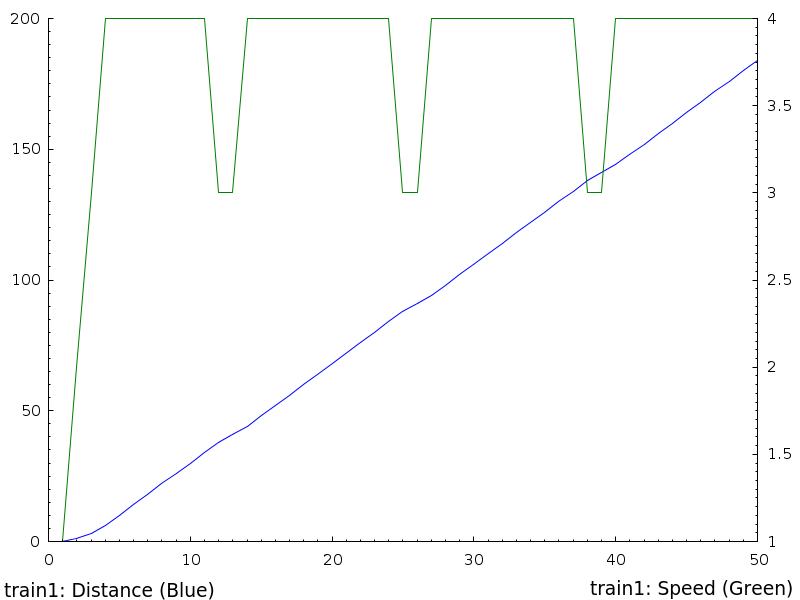
\includegraphics[scale=0.5]{t1graph.png}
\end{center}
\caption{A graph comparing the distance and speed of train1}
\end{figure}

\begin{figure}
\begin{center}
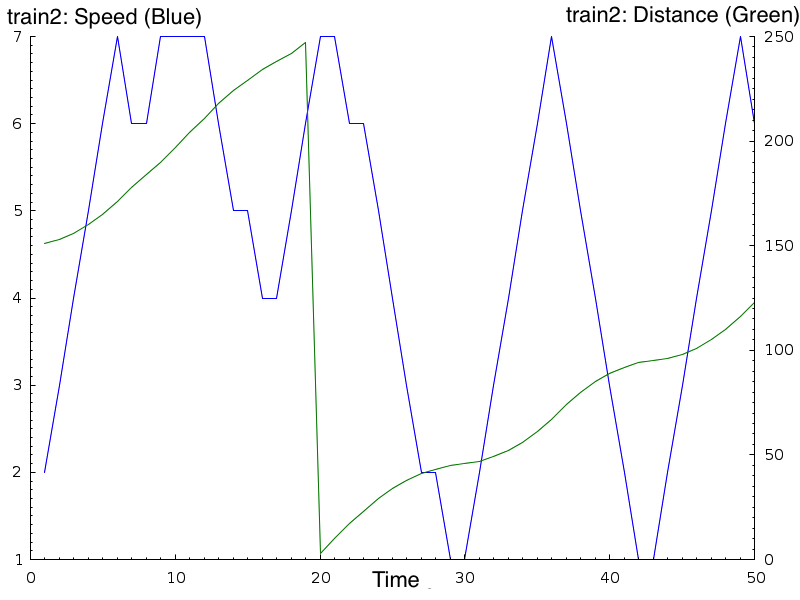
\includegraphics[scale=0.64]{t2graph.png}
\end{center}
\caption{A graph comparing the distance and speed of train2}
\end{figure}

\begin{figure}
\label{t1t2graph}
\begin{center}
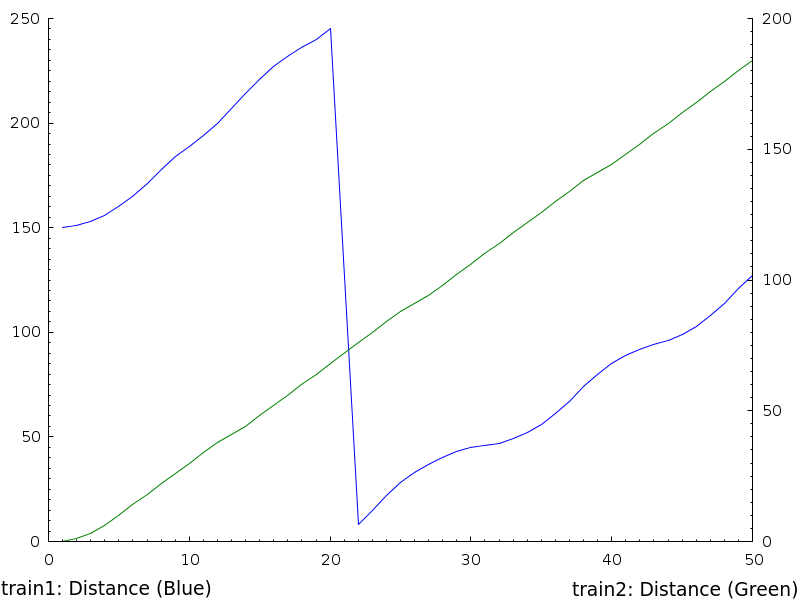
\includegraphics[scale=0.64]{t1t2graph.png}
\end{center}
\caption{A graph comparing the distances of train1 and train2}
\end{figure}

In fig \ref{t1t2} we see that train2 never enters the same track segment as train1.

\section{The Maude Linear Temporal Logic Model Checker}
The Real Time Maude system employs the Maude LTL Model Checker on-the-fly LTL model checker for \cite{ES00} verification purposes.  This is a useful automatic tool which allows for the verification and analysis of real time systems. In addition to the positive verification results in which a safety property holds,  the system produces, in the case of a negative verification result, a counter example trace which describes how the error occured from the initial state of the system.

 

\section{Model Checking the European Rail Traffic Management System}
In the following section we will demonstrate an approach to apply the Real Time Maude LTL model checker to verify the Real Time Maude specification described previously.
Firstly we shall define the property we want to check in the Real Time Maude system. To do this we have to define a satisfaction relation which describes what it means for the property to hold in a state of the system we are checking.  The property we shall consider in this case is that the moment authorities of two trains in system do not overlap. Logical property we define identifies the individual trains using their object identifiers and then computes whether or not an over lap has occurred using a boolean formula.  We shall show that it is possible to verify this property over a time period large enough for all normal behaviours of the system to occur. 

\subsection*{Defining a Satisfaction Relation}
The syntax of the properties for which we are going to check using the LTL model checker are defined separately from the semantics in terms of a satisfaction relation.
We shall now describe how to define the behaviour of the satisfaction relation for a given system and property as a Real Time Maude specification. The satisfaction relation itself is predefined in a specification as an operation which takes a State and a property which is of type Prop and computes a boolean. Maude defines the satisfaction relation $\models$ in the following:
\medskip

\begin{lstlisting}[caption =  The Maude Satisfaction module, label =code:satisfaction ]
  fmod SATISFACTION is  
    protecting BOOL .  
    sorts State Prop .  
    op _|=_ : State Prop -> Bool [frozen] .  
  endfm
\end{lstlisting}
\medskip
The sorts \texttt{State} and \texttt{Prop} are undefined as is the behaviour of $\models$. It is left to the user of the model checker to define the behaviour for their own purposes. The standard way to define predicates which refer to a given object is by matching object identifiers.

We can check that a train is in a specific state as follows:
\begin{lstlisting}[caption = The constant speed property]
ops train-cons : Oid -> Prop [ctor] .
eq {REST < O1 : Train | state : cons >} |= train-cons(O1') 
   = (O1 == O1') . 
\end{lstlisting}
This predicate holds if there is a train in t he configuration with object identifier O1' and a state cons. 

We can check that a train has a certain speed as follows:
\begin{lstlisting}[caption = The speed property]
op train-s : Oid Nat -> Prop [ctor] .
eq {REST < O1 : Train | speed : N1 >} |= train-s(O1',N1') = 
   (N1 == N1') and (O1 == O1') .
\end{lstlisting}

Here the natural number N1 in the train object is matched with N1' in the predicate train-s.

\subsection*{Defining "No Overlapping Movement Authorities"}
We verifying the safety condition "The movment authorities of two trains do not overlap" by model checking two safety properties MA1 and MA2 that correspond to checking the different possible safe positions over movement authorities and trains on the track. To do this we define a satisfaction relation for two Maude operations of type $\mathbf{Prop}$ which capture each of these safety properties. The first of which can be seen below:

\begin{lstlisting}
eq {REST < O1 : Train |  dist : D1 , ma : M1 > 
   < O2 : Train |  dist : D2 , ma : M2 >} |= nomaoverlap1(O1',O2') = 
   (O1 == O1') and (O2 == O2') and noolap1(D1,M1,D2,M2) .
\end{lstlisting}

Here we have matched two object identifiers and natural numbers and called a boolean function \texttt{noolap} on those variables. This definition features an external operation which computes a boolean depending on whether a set of inequalities are satisfied. The two sets of inequalities corresponding to the two safety properties are defined below:

\begin{lstlisting}[caption = The no overlap operations]
eq noolap1(D1,M1,D2,M2) = 
    (D1 <= M1) and (D2 <= M2) implies ((M1 <  D2) or (M2 < D1)) .  
\end{lstlisting}

There are four possible combinations of trains and movement authorities.  The first case is that train one is behind its movement authority which is behind the second train which itself is behind the movement authority. The second case is the reverse of the first case. In the third and fourth cases  one of the trains is behind its movement authority and the other is towards the end of the track and has its movement authority extended into the initial segment at the beginning of the track.


\subsection*{Defining "A Point Does Not Move"}



\subsection{Execution of The LTL Model Checker}
\textbf{Note: do we want to describe and verify other safety conditions here?}
We shall now describe the execution of the LTL model checker in Real Time Maude. This is done using the mc command with some initial state of type system, a satisfaction relation, the LTL formula to be checked and an optional time. The satisfaction relation can be either $\models_u$ for un-timed model checking for which time is not specified or $\models_t$ for which the optional time is specified.

The Real Time Maude LTL model checker is then called using the following command:

\begin{center}
\texttt{(mc initialstate2 |=t [] nomaoverlap(train1,train2) in time <= 30 .)}
\end{center}
The command states that we are applying timed model checking to check that it is globally true that the movement authorities of the trains do not over lap at all moments in time less than or equal to 30. This results in the following output from Real Time Maude which indicates that the property was succesfully verified in 3 minutes and 22 seconds taking the system approximately 140 million rewrites.
\begin{lstlisting}[caption = No overlapping movement authorities model checking result]
rewrites: 138889387 in 179663ms cpu 
(202024ms real) (773054 rewrites/second)

Model check initialstate2 |=t[]nomaoverlap(train1,train2)in 
MODEL-CHECK-ERTMS8 in time <= 30 
with mode deterministic time increase

Result Bool :
  true
\end{lstlisting}

Unfortunately the Real Time Maude LTL model checker can not detect the congruence between difference configurations of control system. Therefore the state space is infinite and it is impossible to do untimed model checking on the above model checking problem for the pentagon example. It is however possible to do timed model checking within a reasonable time limit that allows for all behaviours of the system to be verified. The junction example does not suffer from this problem as the state space is finite and in addition, it has additional mechanisms to remove non-determinism from the model which dramatically cuts down on the state space.


\section{Results}
The following table presents the times taken to verify the 4 safety conditions MA1, MA2, P1 and P2:

 

\section{Conclusion}
 We have presented the first attempt at modelling and verifying the combined ERTMS and interlocking system.
\subsection*{Future Work}
There are numerous ways in which our model can be extended. One of the biggest problems facing engineers when developing the ERTMS system is time and how it affects the transition of messages with delays often occurring. This could be easily be modelled following the work \cite{PO07} where delays are modelled in the communications between nodes of a wireless sensor network. Currently our trains have a jerky behaviour in terms of speed, breaking and accelerating in rapid succession there are several other behaviours that trains exhibit in real life that we have not captured in our model. Trains have the ability to coast where the engine in not powering the train but the brakes are not active which is used for several purposes. To save energy coasting and accelerating are often combined to hold the train at max speed. The trains may also coast before breaking when reaching the end of a movement authority.

Currently the track is closed and trains are capable of looping round the track giving it an infinite state space. Opening up the track with an entrance and exit would provide the opportunity to model the hand over part of the protocol where new trains must register with the RBC on entering the track and then de-register upon leaving. This opening of the track would also finitise the state space possibly allowing for un-timed model checking to take place. This example could then be extended by increasing the complexity of the track further and then modelling routes and points. This would allow for the checking of a further safety conditions that states no train has a movement authority over a point in locked in the wrong direction or a moving point.

The RBC has the possibility to pre-emptively grant movement authorities to trains without them requesting it in the case that a train is on a route which contains free sections of track behind a movement authority.  The trains could also request movement authorities before the point at which we reach the braking point.